\begin{figure}[t]
\centering
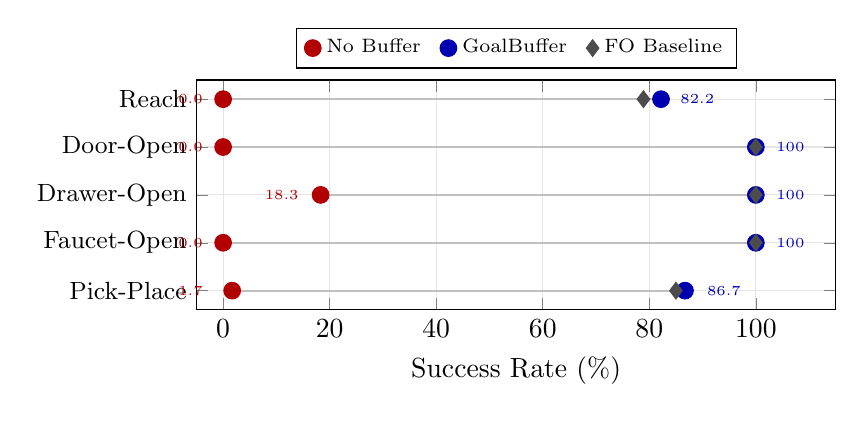
\begin{tikzpicture}
\begin{axis}[
    width=0.8\columnwidth,
    height=4.5cm,
    xmin=-5, xmax=115,
    xlabel={Success Rate (\%)},
    ytick={1,2,3,4,5},
    yticklabels={Pick-Place, Faucet-Open, Drawer-Open, Door-Open, Reach},
    y tick label style={font=\small},
    xtick={0,20,40,60,80,100},
    grid=major,
    grid style={gray!20},
    legend style={at={(0.5,1.05)}, anchor=south, legend columns=3, font=\scriptsize, /tikz/every even column/.append style={column sep=5pt}},
    clip=false,
]
\draw[thick, gray!50] (axis cs:1.7,1) -- (axis cs:86.7,1);
\draw[thick, gray!50] (axis cs:0,2) -- (axis cs:100,2);
\draw[thick, gray!50] (axis cs:18.3,3) -- (axis cs:100,3);
\draw[thick, gray!50] (axis cs:0,4) -- (axis cs:100,4);
\draw[thick, gray!50] (axis cs:0,5) -- (axis cs:82.2,5);
\addplot[only marks, mark=*, mark size=3pt, red!70!black] coordinates {
    (0,5) (0,4) (18.3,3) (0,2) (1.7,1)
};
\addlegendentry{No Buffer}
\addplot[only marks, mark=*, mark size=3pt, blue!70!black] coordinates {
    (82.2,5) (100,4) (100,3) (100,2) (86.7,1)
};
\addlegendentry{GoalBuffer}
\addplot[only marks, mark=diamond*, mark size=3pt, gray!60!black] coordinates {
    (78.9,5) (100,4) (100,3) (100,2) (85,1)
};
\addlegendentry{FO Baseline}
\node[font=\tiny, red!70!black, anchor=east] at (axis cs:-2,5) {0.0};
\node[font=\tiny, blue!70!black, anchor=west] at (axis cs:84,5) {82.2};
\node[font=\tiny, red!70!black, anchor=east] at (axis cs:-2,4) {0.0};
\node[font=\tiny, blue!70!black, anchor=west] at (axis cs:102,4) {100};
\node[font=\tiny, red!70!black, anchor=east] at (axis cs:16,3) {18.3};
\node[font=\tiny, blue!70!black, anchor=west] at (axis cs:102,3) {100};
\node[font=\tiny, red!70!black, anchor=east] at (axis cs:-2,2) {0.0};
\node[font=\tiny, blue!70!black, anchor=west] at (axis cs:102,2) {100};
\node[font=\tiny, red!70!black, anchor=east] at (axis cs:-2,1) {1.7};
\node[font=\tiny, blue!70!black, anchor=west] at (axis cs:89,1) {86.7};
\end{axis}
\end{tikzpicture}
\caption{GoalBuffer recovery under WeakPO. Each line spans from No Buffer (red) to GoalBuffer (blue); gray diamonds mark the FO baseline. A zero-cost goal cache lifts WeakPO success from 0--18.3\% to 82.2--100\%, often matching FO.}
\label{fig:goalbuffer}
\end{figure}
